\section{Artiphishell's Architecture}
\label{architecture}

Artiphishell has an agent-based architecture, in which various components (agents) with specific tasks collaborate in order to carry out the overall task of finding and patching vulnerabilities.
The overall architecture of Artiphishell is shown in Figure~\ref{architecture}.

\begin{figure*}[h]
  \centering
  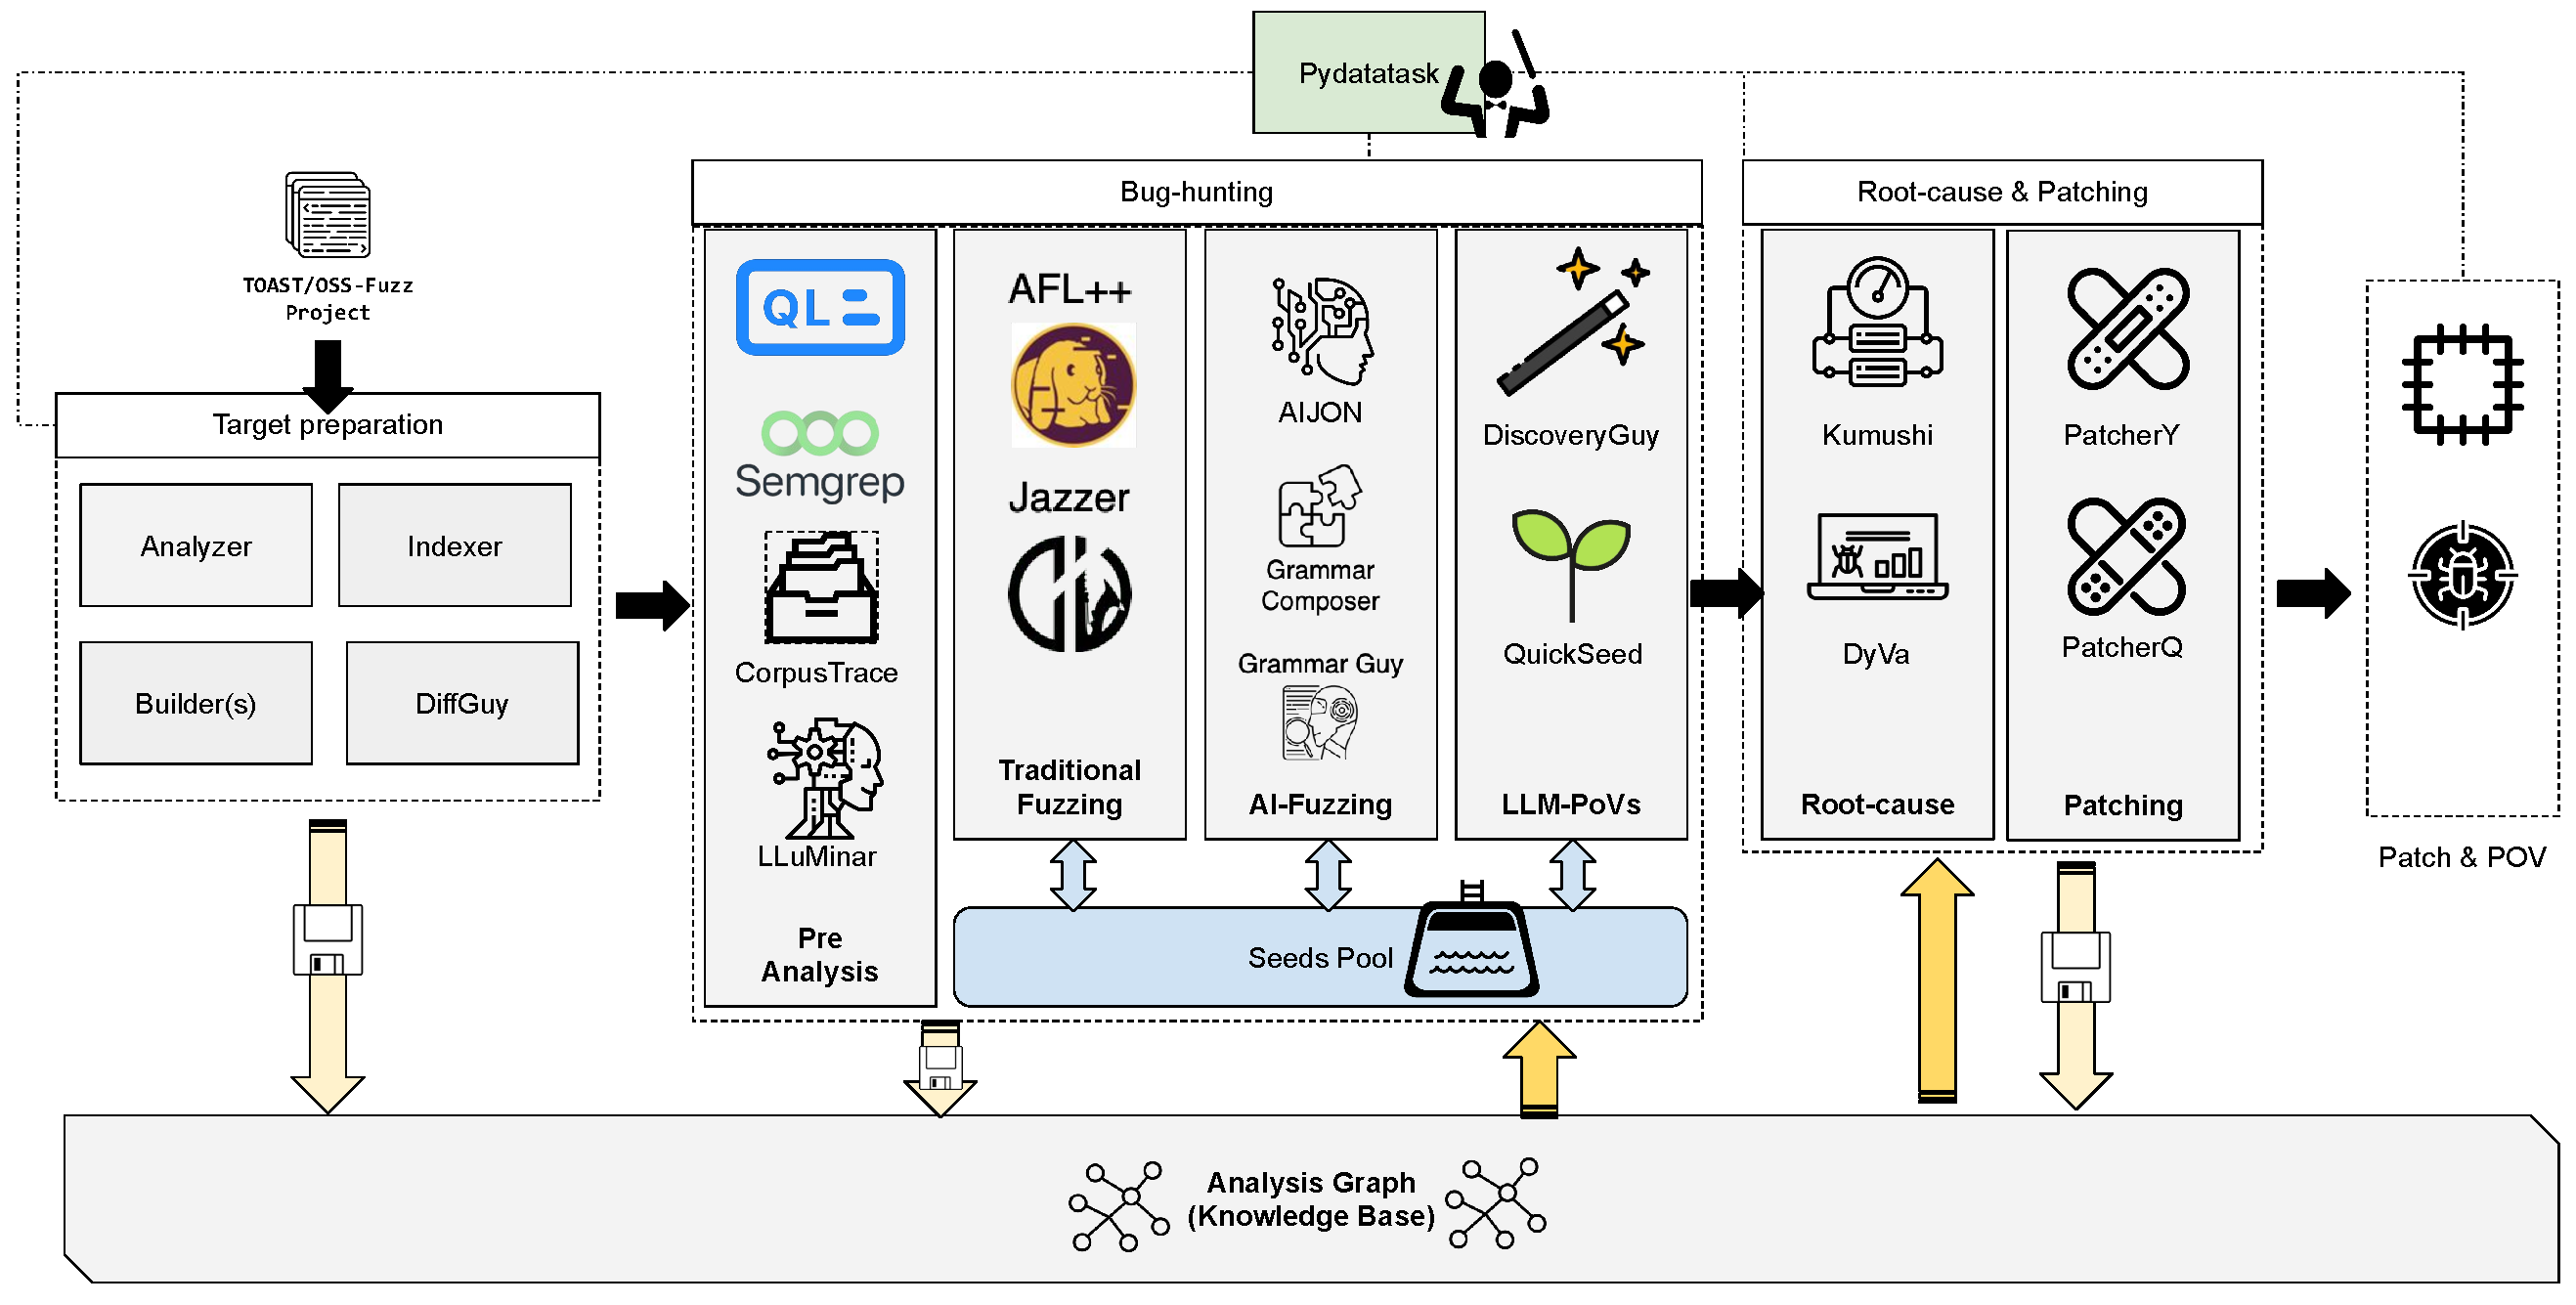
\includegraphics[width=\linewidth]{figures/artiphishell.pdf}
  \caption{The Artiphishell architecture.}
  \label{fig:architecture.}
\end{figure*}


\subsection{ARTIPHISHELL Pipeline Architecture \& Data Model}

ARTIPHISHELL is implemented as a dataflow pipeline in which components are launched on-demand as soon as the data they depend on is available (if sufficient resources are available).
E.g. fuzzing tasks would depend on build artifacts that are created by build tasks that in turn depend on the target source code and the project metadata. The build task will launch first, while the fuzzing task will remain blocked until the build task has completed and uploaded the build artifact.

This pipeline is backed by our orchestration framework \textit{pydatatask} which consists of two main services: the agent and the runner.
The agent handles data storage on various backends (e.g. S3 buckets, local file system, cached layers, etc.) as well as dynamic delivery and retrieval of pipeline data to components over HTTP.
The runner periodically queries the agent to retrieve the current state of the pipeline and handles tasking, scheduling, preemption and auto-scaling of pipeline tasks.

Throughout the competition, ARTIPHISHELL in its pipeline handles various types of data which can be stratified in two ways.
Firstly, they can be grouped by the type of the data stored: folders of files shipped as tar archives, single files in the form of binary blobs and parseable metadata in YAML or JSON format.
In \textit{pydatatask}, their repositories are referred to as FilesystemRepository, BlobRepository and MetadataRepository, respectively.
For example, build artifacts are folder structures which are stored in a FilesystemRepository, whereas crashing seeds are stored in a BlobRepository with an associated MetadataRepository which describes the origin of the crashing seed.

Secondly, the data in the pipeline can generally be clustered into the following semantic groups:

\begin{itemize}
    \item Source Code Repositories
    \item Build artifacts
    \item Static Analysis Results + Rankings
    \item Code Indexing Results (Split functions, identifiers, globals, etc.)
    \item Fuzzing grammars (Nautilus) + Serialized Grammar Derivation Trees (referred to as RONs) + Dictionaries
    \item Harness inputs (Seeds + crashes)
    \item Crash Reports + Triage Reports
    \item Generated patches
    \item SARIF reports (both generated by ARTIPHISHELL as well as provided by the organizers in tasking)
    \item Submission tasking + artifacts
\end{itemize}

Data in repositories can be accompanied by additional metadata.
This metadata is used to allow components to track the origin of said data (e.g. which component produced a given crash),
as well as to associate additional data from different stages, e.g., linking a crashing seed with both the harness
it was discovered for as well as the sanitizer that the crash occurs with.

While most of this data is transferred and maintained by the agent of our orchestration framework, pydatatask, more ephemeral
pieces of data, e.g. fuzzing seeds, grammars and fuzzing dictionaries are purely managed by \seedsync and maintained and processed solely on fuzzing nodes.
Nonetheless, we also upload a "canonical representation" of these findings in the pydatatask agent itself, e.g. by marking a single fuzzing instance as the "representative" instance.
This allows components at all stages of the pipeline to use this information, while avoiding the upload of redundant data.


\subsection{Orchestration}

The steps outlined above are carried out by a group of autonomous agents that are coordinated by the \orchestrator component.
The \orchestrator uses a purpose-built framework, called \pydatatask, which allows one to specify the data dependencies between the various agents and the ordering constraints on their execution.

The \orchestrator is also in charge of distributing the task to achieve the best possible use of the available computing resources, as well as control over the strategy to optimize the outcomes within the constraints and scoring rules of the AIxCC competition.
Figure~\ref{fig:orchestrator} shows a snapshot of the \orchestrator's monitoring interface, which shows the various agents and their interconnections.

\begin{figure*}[h]
  \centering
  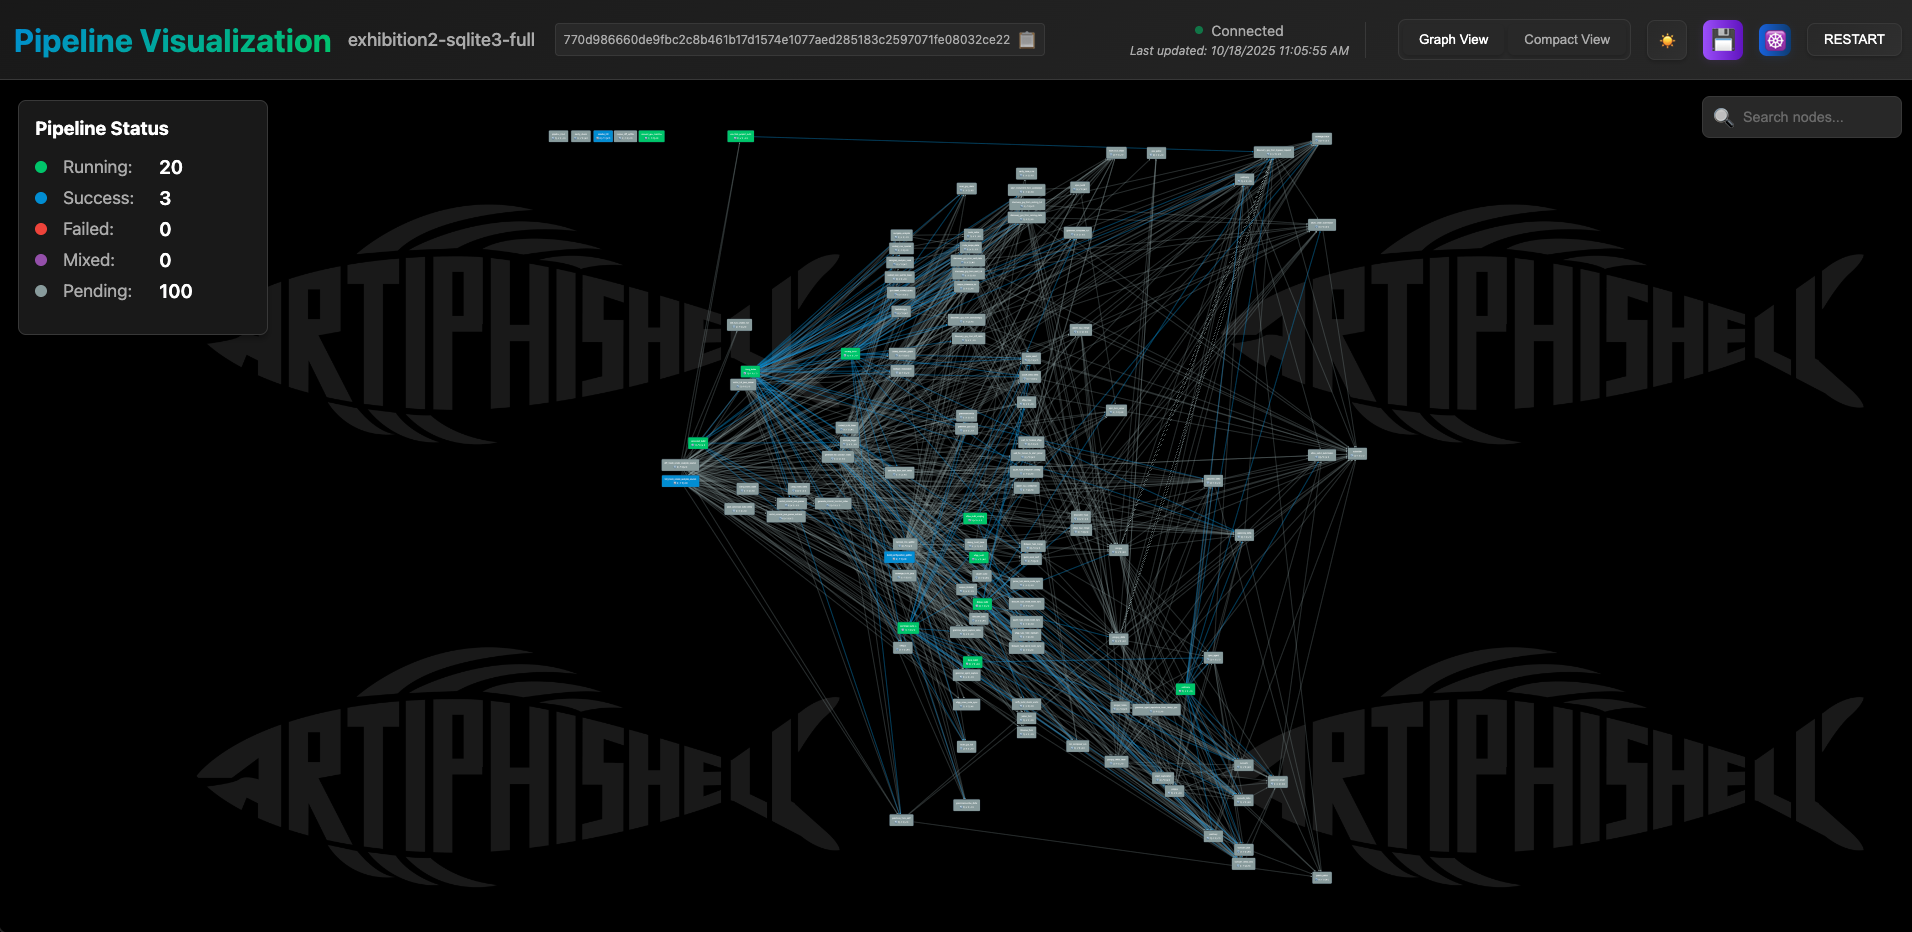
\includegraphics[width=\linewidth]{figures/pdviz.png}
  \caption{The \orchestrator's monitoring interface.}
  \label{fig:orchestrator}
\end{figure*}

\subsection{Inputs}

The system takes as input the source code of an application in The Open Application Security Testing (TOAST) format~\cite{aixcc:toast}, which is identical to the format used by OSS-Fuzz.
The target application can be provided in either \emph{full mode} or \emph{delta mode}.

In full mode, the application is provided in its entirety, and the task of the CRS is to identify vulnerabilities and provide patches for them.
This scenario mimics the use case where an existing code base is analyzed for possible vulnerabilities.

In delta mode, the application is provided as a base version together with a series of changes that have been applied to the code. 
In this case, the CRS must find vulnerabilities that have been introduced through these specific changes: that is, each identified vulnerability must be paired with the specific change that introduced it.
This mode models the use-case scenario in which developers have introduced changes to an existing code base, and it is desirable to review the added code to avoid the introduction of new bugs.

\subsection{Preprocessing}

\artiphishell applies to the target application a preprocessing step that includes building several versions of the application and extracting meta-information about the source code base, such as the Control Flow Graph (CFG), the Code Property Graph (CPG), the location of each function in the code base, as well as the strings contained in the application. 
These artifacts and the corresponding meta-information are stored in several shared repositories that are accessed by the agents responsible for vulnerability analysis and patching.

Note that while the results of this initial preprocessing step are used by several subsequent analyses, there are agents that will start their job with limited information (i.e., before some of the preprocessing is terminated), in an attempt to optimize time and resources.
This is required by the structure of the AIxCC competition, which includes time-limited runs, and would be handled differently if timing were not a limiting issue.

\subsection{Points of Interest}

An important step in the analysis is to determine which locations of the target application code base are the most likely to contain bugs.
Past research has demonstrated that sometimes locations of ``problematic code'' can be identified by code smells~\cite{Neuhaus2007}, complexity analysis~\cite{Moshtari2013}, and even past repository history~\cite{meng2021:Bran}.
\artiphishell uses a combination of static analysis, heuristics, and LLM-based techniques to identify which functions are more likely to contain vulnerabilities.
In addition, for targets in delta mode, the points of interest are directly associated with the location of the changes, and this phase integrates this information with the other analyses to provide an overall ``heat map'' of the code base.

\subsection{Vulnerability Analysis}

Vulnerability analysis includes the steps of vulnerability identification, vulnerability verification, and crash deduplication.
Vulnerability identification is performed by a set of agents that use both static and dynamic analysis techniques to find inputs that cause security violations.

Security violations are detected by \emph{sanitizers}, which monitor code execution and identify abnormal conditions.
For example, a sanitizer might detect faulty memory accesses and generate an alert whenever a program pointer references an address that has not been allocated to the process, as, for example, in a null pointer dereference.
In this case, the process is terminated and a report is generated. 
The reports created by sanitizers contain important meta-information that supports the root cause analysis and patching of the bug.

These reports include the input that caused the violation, the harness that processed the input, and one or more stack traces that represent the status of the program at key points during the execution.
For example, a use-after-free violation might include a stack trace for the point at which the memory was allocated, a stack trace for the location where the memory was freed, and a stack trace for when the pointer to the free memory was used.
Once a crashing input is identified, the following step is to verify that the input reliably triggers the sanitizer, to avoid imprecision due to nondeterminism.

Once the input passes this test, the crash information is passed to a deduplication component, whose task is to determine if this particular crash is similar to crashes that have been previously found.
In general, this is a step performed by most vulnerability analysis processes based on fuzzing, as crashes caused by the same root cause can be triggered by multiple inputs.
However, in the context of the AIxCC competition, this step is especially important, as submitting multiple inputs that are judged to trigger the same bug has a negative impact on the final score.

The final output of this phase is a ``proof of vulnerability'' (PoV) that demonstrates reliably how an input to one of the harnesses of the application can cause the triggering of a sanitizer.

\subsection{Root Cause Analysis}
Once a unique crashing input has been identified, the next step is to generate a patch that prevents the crash.

The patch should prevent the exploitation of the vulnerability without changing the overall functionality of the application; that is, for all non-crashing inputs, the behavior of the application should be the same for both the original and patched applications.

However, the generation of effective patches is an open problem that does not have a general solution, because of a number of challenges.
First of all, it can be challenging to determine the actual root cause of a vulnerability because abnormal behavior experienced at a certain point in the execution of the program might actually be caused by events that happened in a different location.
Consider, for example, an integer overflow that causes an array index to be out of bounds.
The conversion of the integer that caused a small negative integer value to be interpreted as a very large value will not cause a crash until the index is used as an offset from the array base pointer at a specific location.
A patch that checks the array index when it is used in this location might not be effective if there are other locations where the index might be used.
In this case, an effective patch would be one that prevents the erroneous conversion of the index, since this is the actual root cause of the bug.

\artiphishell uses a composition of traditional analysis techniques and LLM-based agents to identify the root cause of vulnerabilities.
For example, dedicated root-cause-analysis components look at the stack trace contained in a crash report and try to identify the functions that are most likely to contain the bug.
In addition, agents equipped with debugging tools use interactive analysis to recover the actual location where a bug is introduced.
In both cases, the output of this phase is the generation of a list of functions that are likely to contain the root cause of the crash.

\subsection{Patching}

\artiphishell uses LLM-based reasoning in order to identify possible patches for the functions that have been identified as likely to contain the root cause of a crash.
Once a patch is identified, a verification process is started in an attempt to bypass the patch to increase confidence in the patch's ability to cover all possible cases.
Once a patch is generated, it is submitted to evaluator components together with the proof-of-vulnerability.

\subsection{SARIF Report Analysis}
The CRSs in the AIxCC competition are required to process vulnerability reports generated by static analysis tools in the SARIF format~\cite{sarif}.

Specifically, CRSs must determine whether each organizer-provided report describes a true positive or a false positive. If the vulnerability is confirmed, they must also produce a patch to fix it.

\artiphishell adopts a two-step strategy to evaluate SARIF reports.
First, it leverages an LLM agent (conveniently named as \emph{SarifGuy}) to open the relevant files and verify the presence of vulnerable code at the reported location. If the agent confirms the vulnerability, it marks the report as a true positive; otherwise, it classifies it as a false positive.
In the second step, a secondary agent attempts to generate a crashing input at the location specified in the report. If the agent succeeds in producing such a seed, the assessment is either updated to true positive (if previously marked false positive) or retained as true positive.

Notably, in \artiphishell, the assessment process is unidirectional: a report’s status may transition from false positive to true positive, but once it is classified as a true positive, this verdict is never reverted. In other words, failing to generate a crashing seed after an initial true positive assessment does not provide sufficient evidence to invalidate the original classification.


%LLM-based agents to perform these tasks.
%In particular, it uses the information collected during the processing of the target application to contextualize the report and produce a crashing seed.
%In addition, it uses the same process used to patch discovered vulnerabilities to attempt patching the flaw.

\medskip

In the following sections, we provide additional details on the components that carry out the phases of the vulnerability discovery and patching process.